\chapter{Implementation}
\label{chap:opendial}

\note{CHAPTER NOT READY YET!!}

This chapter exposes the most important features of the \opendial toolkit, which is a Java-based software toolkit developed to design and evaluate dialogue systems based on probabilistic rules. The toolkit implements all the data structures and algorithms detailed in this thesis.  It also served as a experimental platform to carry out the empirical studies presented in Chapters \ref{chap:wozlearning}, \ref{chap:rllearning} and \ref{chap:user-evaluation}. 

The chapter is divided in three sections.  The first section summaries the most important characteristics of the dialogue architecture and surveys the system modules integrated in the system and the graphical user interface developed to monitor and control the system state.  Section \ref{sec:domain-specification} focuses on the declarative specification of the probabilistic rules for the domain. Section \ref{sec:corealgorithms} then discusses a range of technical questions related to the implementation of algorithms related to approximate inference, sampling, and forward planning. Finally, Section \ref{sec:archi-comparison} compares \opendial to other architectures developed in dialogue systems research. 

\section{Architecture}
\label{sec:genarchitecture}

\subsection{General workflow and scheduling}

he dialogue system developed for this thesis relies on a blackboard, event-driven architecture. As already mentioned throughout this thesis, blackboard architectures are widely used in spoken dialogue systems for their ability to handle flexible workflows where multiple modules ``cooperate'' to  interpret the user inputs, maintain a representation of the current situation, and decide on the best actions to perform. Information-state approaches are notably based on such system architecture \cite{Larsson:2000:ISD:973935.973943}. In dialogue domains, the blackboard represents the dialogue state. The system modules are in charge of updating this dialogue state in accordance with the recognised user utterances, perceived contextual changes, and selected system actions. 

Figure \ref{fig:impl_architecture} provides a high-level illustration of the workflow corresponding to such architecture. One can easily note from the figure that the dialogue state stands at the center of the workflow. The system modules can both read (dashed arrows) and write (plain arrows) to this dialogue state.  The scheduling of these processing operations is done in an event-driven manner. After each change, the dialogue state sends an event message to all its attached modules to inform them that the state has been updated. The modules can subsequently react to this update by generating new updates.  The process continues until the dialogue state stabilises.  


\begin{figure}[h]
\centering
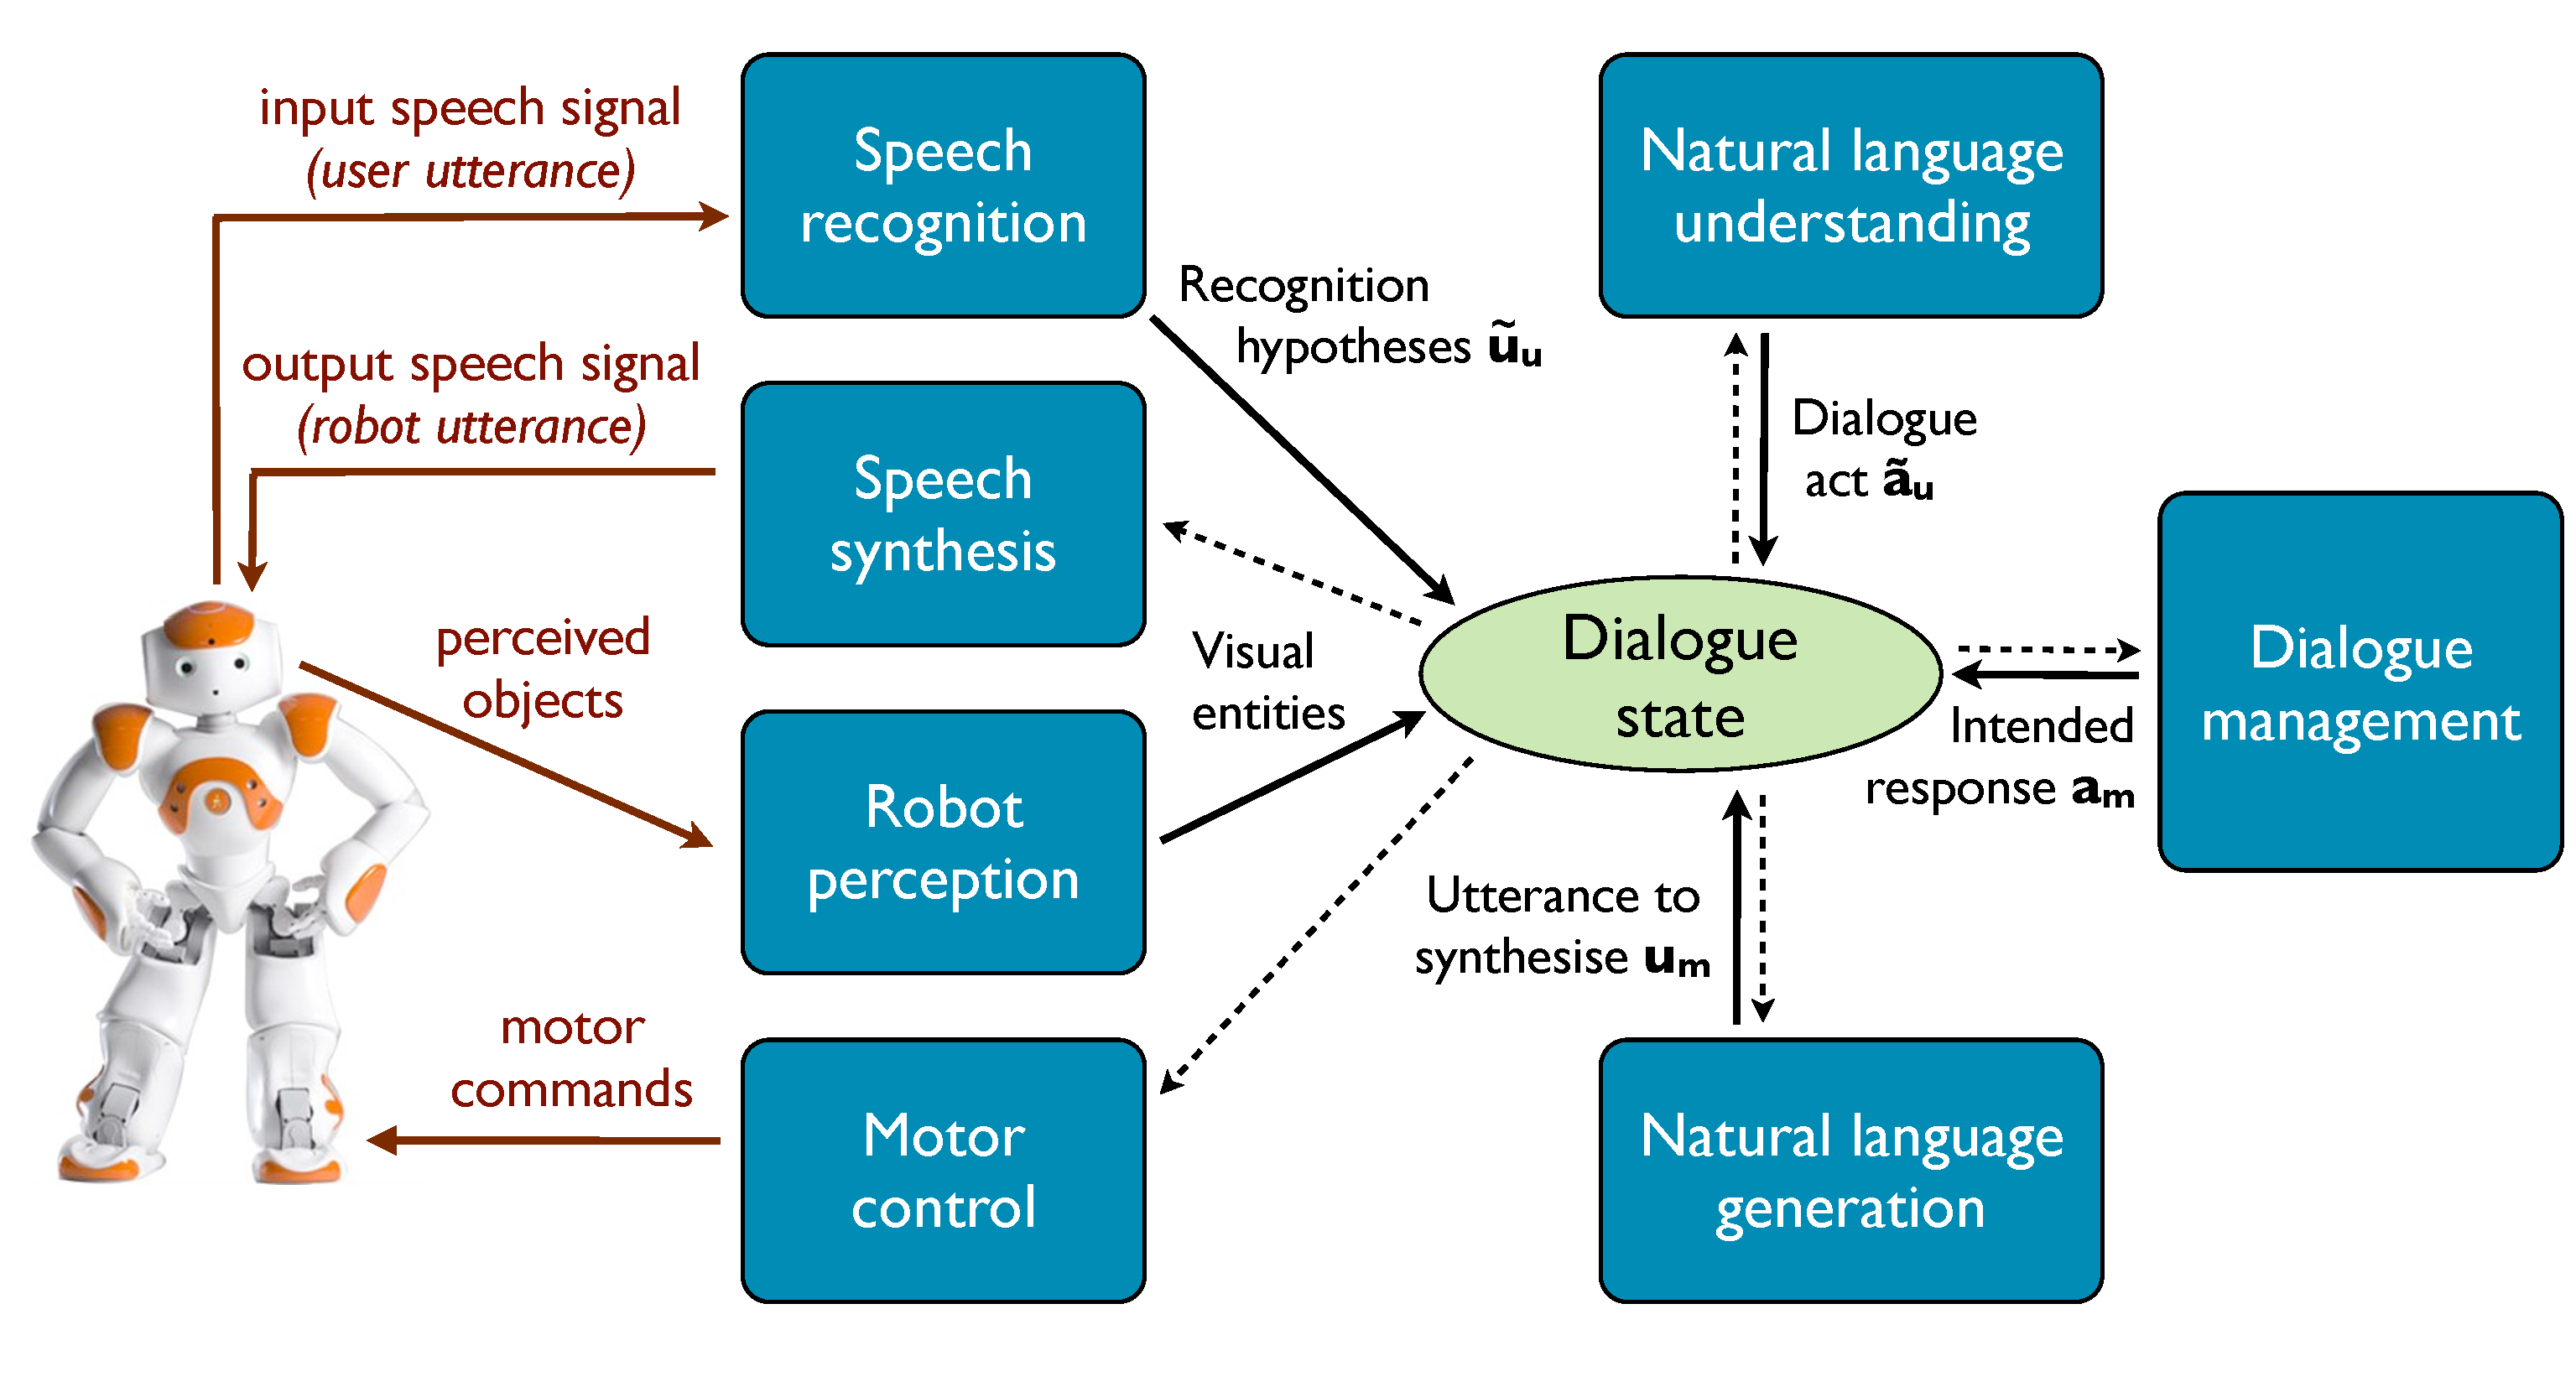
\includegraphics[scale=0.30]{imgs/impl_architecture.pdf}
\caption{Generic system architecture employed in this thesis.}
\label{fig:impl_architecture}
\end{figure}

The \opendial toolkit allows system modules to run in parallel, using Java multi-threading. The possibility to execute modules in parallel is particularly useful in dialogue architectures, as the system must be able to react to user input and contextual changes occurring at any time -- even while other modules are still busy processing a previous update.  Many of the modules developed in the toolkit (such as planning and probabilistic inference) can also operate in anytime mode, which implies that they can be interrupted at any time and still provide an output. 

The current implementation of \opendial is optimised to run on a single platform.  System modules can however remotely connect to external resources on the robotic platform to perform various tasks related to robot perception and motor control. Given the blackboard architecture of the toolkit, the framework could however be extended to support fully distributed systems in the future.

\subsection{System modules}

System modules can operate in either synchronous and asynchronous mode: \begin{itemize}
\item Synchronous modules continuously monitor the dialogue state for relevant changes.  Their activation is thus in synchrony with the update events generated by the dialogue state.
\item Asynchronous modules run independently of the dialogue state.  They typically relate to visual or speech perception tasks. When new observations are made, they update the dialogue state with the corresponding information.
\end{itemize}

All modules have access to the complete dialogue state and can therefore exploit the full set of state variables (including generic contextual information) in their processing. We review below the modules shown in Figure \ref{fig:impl_architecture} and describe their role and internal structure. It should be emphasised that the focus of the present thesis is on dialogue management.  The other system modules are therefore deliberately limited to simple, ``shallow'' processing methods in order to concentrate the implementation efforts on the dialogue manager. Many of these modules could however be extended to employ more sophisticated techniques, in particular in regard to speech recognition, natural language understanding and generation. 

\subsubsection*{Speech recognition}

Speech recognition is performed on the robot platform, using a commercial, off-the-shelf speech recognition engine (Vocon 3200 from Nuance).  Four microphones placed on the robot head are used for the sound capture.  The positioning of the microphones on the robot allows the user to interact with the robot in a natural manner, without needing to resort to head-mounted microphones. This increased naturalness comes however at the price of a degraded sound quality due to the larger (and varying) distance between the sound source and the microphones, combined with the presence of noisy mechanical motors at only a few centimetres from the sound capture.

The acoustic model employed in all experiments was provided along with the speech recognition engine, and was optimised for American English. The language model takes the form of context-free recognition grammars specified in Bachus-Naur Form (BNF). Distinct grammars were used to cover the domain of discourse of each experiment. The grammars were designed by hand, based on the Wizard-of-Oz transcripts collected in our empirical studies (cf. previous chapters). Grammars can be dynamically attached or removed from the engine at runtime, thereby allowing the system to adapt the recognition to the current dialogue context. This functionality is however not yet exploited in the current architecture (but see e.g. \cite{ESSLLI2008-springerreprint} for a description of our prior research work on this issue). As the recognition engine only generates hypotheses with raw (unnormalised) confidence scores, a normalisation routine was implemented to transform them to a proper probability distribution $P(\tilde{u}_u)$.\footnote{The conversion between confidence scores and probabilities is manually tuned in the current implementation.  Future work may however rely on more principled estimation techniques such as the ones outlined in \cite{Williams08}.}


\subsubsection*{Natural language understanding}

The goal of natural language understanding (NLU) is to map a collection of utterance hypotheses $\tilde{u}_u$ to a related set of dialogue act hypotheses $\tilde{a}_u$ expressing the semantic and pragmatic content of the user input. This understanding step is decomposed in our implementation in two tasks, dialogue act recognition and visual reference resolution.  

The goal of dialogue act recognition is to construct the logical form representing the meaning of the utterance. It should be noted that a user utterance may contain more than one dialogue act, as for instance in \utt{yes and now pick the blue object}.  A collection of domain-specific templates was designed by hand to convert surface forms into logical representations of dialogue acts.  Although this approach does not allow for ``deep'' semantic extraction, it was shown to perform well in our dialogue domains. Future work may replace this template-based method with a data-driven semantic parser based on e.g.  dependency parsing \citep{Nivre:Etal07}.  

Reference resolution is used to map linguistic expressions referring to objects in the visual context to their corresponding object identifier.  This mapping is two steps.  First, the properties stated in the linguistic expressions are matched against the set of possible references.  In case the description remains ambiguous (i.e. more than one object matches the linguistic expression), the references can be further ranked according to their visual saliency, defined here in terms of their physical distance to the robot. 

Natural language understanding is practically implemented in \opendial via probabilistic rules.  As seen in Section \ref{sec:amodelling}, the formalism of probabilistic rules already includes special-purpose operators for string manipulation and can thus readily encode the shallow templates used for dialogue act recognition.  Rule $r_{15}$ below is an example of such rule.  The rule lists three regular expression patterns associated with the dialogue act $\mathrm{MoveArm(Left,Down)}$.  If the value for the user utterance variable $u_u$ matches at least one of the patterns, the dialogue act $a_u$ is classified as $\mathrm{MoveArm(Left,Down)}$:
\begin{align*}
r_{15}: &\;\;\textbf{if} \ (u_u \textit{ matches } \text{`` (*) left arm down''} ) \\ 
& \lor (u_u \textit{ matches } \text{`` (*) lower (the\,|\,your) left arm''} ) \\
& \lor (u_u \textit{ matches } \text{`` (*) down (the\,|\,your) left arm''}   )  \ \ \textbf{then} \\ 
& \; \; \begin{cases} P\left(a_u = \mathrm{MoveArm(Left,Down)}\right) = 1.0 \end{cases}
\end{align*}

\subsubsection*{Dialogue management}

Dialogue management follows the procedure outlined in Section \ref{sec:processing-workflow} and will thus not be repeated here. After a dialogue state update, the dialogue manager triggers the corresponding rule-structured models, and selects the next action to perform (if any). 

\subsubsection*{Natural language generation}

If the selected system action is non-empty and corresponds to a verbal action, the natural language generation module is triggered.  As for natural language understanding, the generation component of \opendial is based on a manually designed collection of templates, but are here applied to convert a logical representation of the communicative goal into a surface form. 

As for natural language understanding, the generation templates are also encoded with probabilistic rules -- although this time the rules are utility rules, since generation is a decision-making task.  As an example, rule $r_{16}$ generates the system response $u_m$ given the system act $a_m=\mathrm{Acknowledgement}$.  The rule specifies in this case three alternatives with equal utility:
\begin{align*}
r_{16}: &\;\;\textbf{if} \ (a_m = \mathrm{Acknowledgement} )  \ \ \textbf{then} \\ 
& \;\; \begin{cases} U(u_m'=\text{``ok''}) = 1 \\ U(u_m'=\text{``great''}) = 1 \\ U(u_m'=\text{``thanks''}) = 1 \end{cases}
\end{align*}

The presence of multiple realisations allows for some variation in the system behaviour, since the system will automatically select one realisation at random (due to the equal utility assigned to the alternative realisations).

\subsubsection*{Speech synthesis}

Speech synthesis is performed on the robot, using an off-the-shelf speech synthesis engine developed by Acapela\footnote{\begin{scriptsize}\url{http://www.acapela-group.com}\end{scriptsize}}. The synthesis engine is based on unit selection. The output speech signal is then sent to two speakers placed on the robot head. To avoid spurious recognition results, the speech recognition is automatically disabled when the robot is speaking.   
 
\subsubsection*{Robot perception}

The robot can detect simple physical objects present in the visual scene. The object detection is done based on the vision libraries bundled with the robotic platform. Special markings are placed on top of the objects 
to facilitate the detection and the visual servoing. 

\subsubsection*{Robot motion control}

Various types of robot movements were employed in our experiments, including both generic body movements (rotating the arms and the head in various directions), spatial navigation (moving forward and backward, turning left and right) and object manipulation (grasping and releasing objects).  All the movements were programmed by hand, using the motion control libraries on the robot. 

\subsection{Graphical user interface}

The graphical user interface developed for the \opendial toolkit allows the system designer to monitor and control in real-time the current state of the system.  The interface is divided in two alternative views, shown as distinct tabs in the application window: the chat window and the dialogue state monitor.

\subsubsection*{Chat window}
The chat window presents the interaction history as a chat window.  The user inputs are shown as N-best lists together with their corresponding probabilities.  Figure \ref{fig:gui-chatbox} provides a screenshot of the chat window. 

In addition to monitoring the interactions, the chat window can also be used to test the dialogue system by typing new user and system inputs in the input field at the bottom of the window.  The agent role can be switched in the drop-down field in the bottom right corner. 

\begin{figure}[h]
\centering
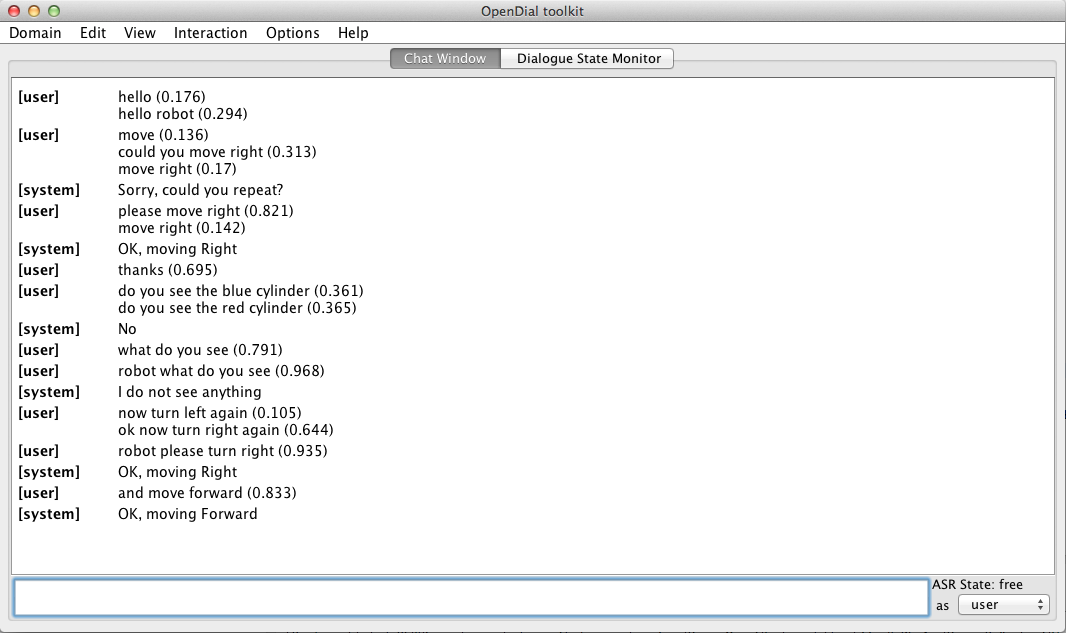
\includegraphics[scale=0.40]{imgs/gui-chatbox.png}
\caption{Graphical user interface showing the interaction history.}
\label{fig:gui-chatbox}
\end{figure}

\subsubsection*{Dialogue state monitor}

To allow the system designer to inspect the content of the dialogue state, a visualisation tool has also been integrated into \opendial .  The tool draws a graph with nodes corresponding to the state variables and directed edges corresponding to conditional dependencies.\footnote{The graphs are rendered using JUNG, which is a Java-based open source toolkit for drawing various kinds of graph structures -- cf. \begin{scriptsize}\url{http://jung.sourceforge.net}\end{scriptsize}.} An example of graph layout is shown in Figure \ref{fig:gui-bn}. The graph is dynamically refreshed after each update of the dialogue state. The graph layout is automatically calculated to optimise the visualisation. 

In addition to showing the current dialogue state, the dialogue state monitor can also record and store previous dialogue states.  The dialogue state to visualise can be selected among the list on the left side of the window. This functionality is useful to e.g. compare dialogue states with one another and analyse how the dialogue state is evolving over time. 

\begin{figure}[h] 
\begin{center}
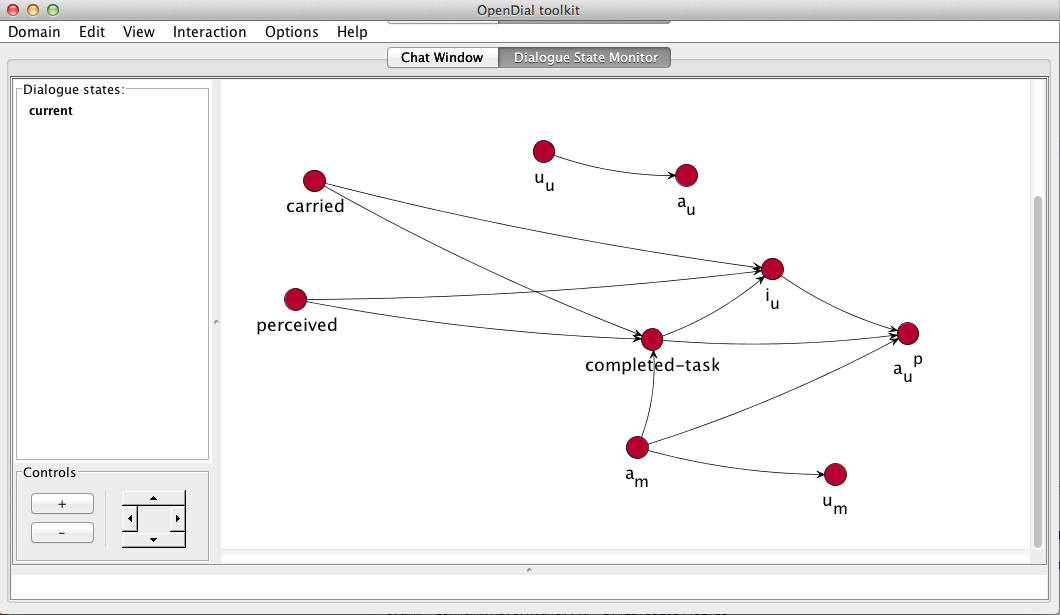
\includegraphics[scale=0.40]{imgs/gui-bn.png}
\end{center} 
\caption{Visualisation of the current dialogue state.}
\label{fig:gui-bn}
\end{figure}

The graph can be manipulated in multiple ways in order to e.g. inspect the content of specific state variables, add or remove evidence, or request the calculation of marginal distributions on selected set of variables.  The inference results are shown in the text area at the bottom of the window.  In addition, the system designer can also directly view the shape of selected probability distributions using the distribution viewer tool illustrated in Figure \ref{fig:gui-distribviewer}. Discrete probability distributions are shown as histograms, while continuous probability distributions are graphically represented by their probability density functions.\footnote{The graphical rendering of the probability distributions is done with the open source toolkit JFreeChart, cf. \begin{scriptsize}\url{http://jfreechart.sourceforge.net}\end{scriptsize}.} 


\begin{figure}[h] 
\begin{center}
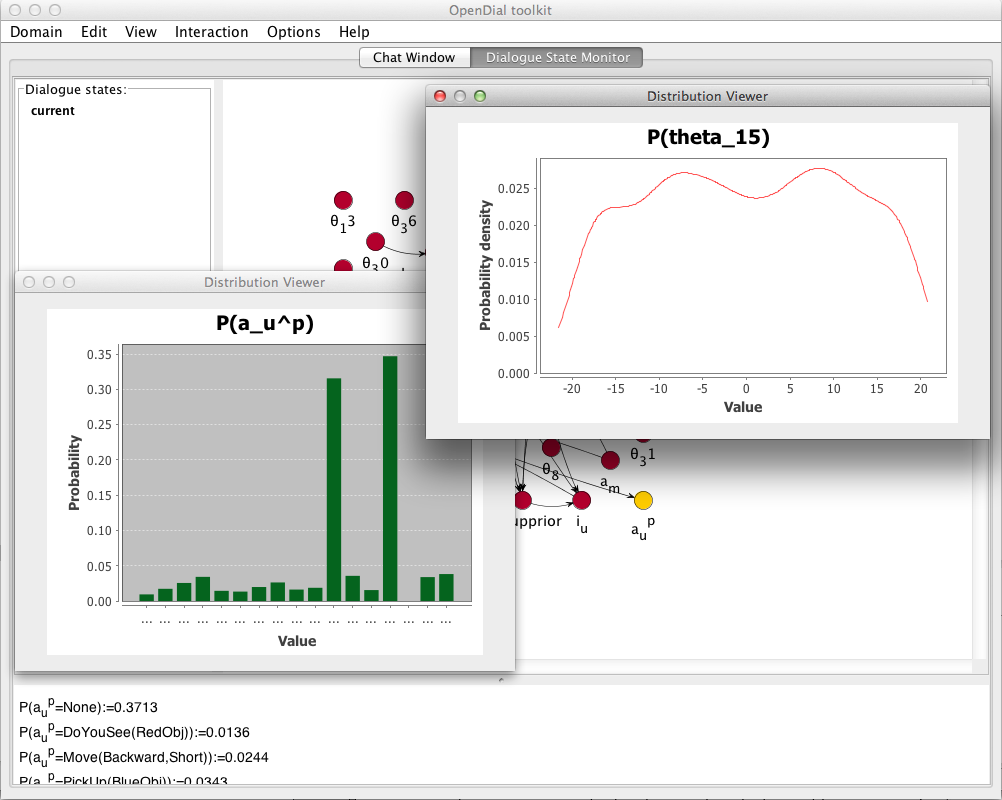
\includegraphics[scale=0.40]{imgs/gui-distribviewer.png}
\end{center} 
\caption{Distribution viewer showing both a discrete probability distribution for $P(a_u^p)$ and a continuous probability distribution $P(\theta_{15})$.}
\label{fig:gui-distribviewer}
\end{figure}

\section{Specification of dialogue domains}
\label{sec:domain-specification}

\subsection{Motivation}

Many reasoning tasks can be structured in terms of probabilistic rules.  As we have seen in the previous section, probabilistic rules have also been applied to natural language understanding and generation tasks in addition to dialogue management. The dialogue domain designed for the user experiments in Chapter \ref{chap:user-evaluation} included for instance a total of 6 models: one dialogue act classification model, (triggered by the user utterance $u_u$), one action utility model (triggered by the user dialogue act $a_u$), three probability models to predict the effects of the system action on the context, the user intention and the next user action (all triggered by the system action $a_m$), and a generation model (triggered by the system action $a_m$).  The association of trigger variables to the rule-based models provides a simple and flexible a way to define the processing pipeline for the application.  Variables can function as triggers for more than one model, allowing models to be instantiated in parallel.

As argued in \cite{lison-semdial2012}, the expressive power of probabilistic rules allow them to capture the structure of many dialogue processing tasks.  Compared to traditional architectures in which the components are developed separately and rely on ad hoc representation formats, the use of a shared formalism to encode the domain models yields several advantages:
\begin{description}
\item [Transparency: ] The reliance on a common representation format provides a unified, transparent semantics for the dialogue state, since all state variables are described and related to one another through a principled framework grounded in probabilistic modelling.  This makes it possible to derive a semantic interpretation for the dialogue state as a whole -- in terms e.g. of a joint probability distribution over the state variables. 

\item [Domain portability: ]  As all domain-specific knowledge is declaratively specified in the rules, the system architecture is essentially reduced to a generic platform for rule instantiation and probabilistic inference.  This declarative design greatly enhances the system portability across domains, since adapting a system to a new domain only requires a rewrite or extension of the domain-specific rules, without having to reprogram a single component.  This stands in sharp contrast with ``black-box'' types of architectures where much of the task- and domain-specific knowledge is encoded in procedural form within the component workflow.

\item [Flexible workflow: ] Probability rules can design very flexible processing pipelines where state variables are allowed to depend or influence each other in any order and direction.  Models can be easily inserted or extended without requiring any change to the underlying platform. Furthermore, several models can be triggered concurrently on the same input/output variables.\footnote{Output distributions can indeed handle effect specifications arising from multiple, sometimes conflicting sources, as we have seen in Section \ref{sec:probruleinstantiation}.} This allows the system to take advantage of multiple, complementary modelling strategies while ensuring that the dialogue state remains consistent. 

\item [Joint optimisation: ] Finally, the use of a unified modelling formalism allows domain models to be optimised jointly instead of being tuned in isolation from one another. Joint optimisation has recently gained much attention in the dialogue system community to overcome the fragmentation of current system architectures and attempt to directly optimise the end-to-end conversational behaviour of the system \citep{Lemon:2011}. 

\end{description}

It should be noted that the architecture does not in any way preclude the integration of other types of processing modules in addition to rule-structured models, as long as these modules can read and update the dialogue state when relevant changes are detected. 

\subsection{Encoding format}

Probabilistic rules are encoded in an XML format with a specifically designed syntax. Listing \ref{listing:xml1} illustrates an example of probability rule encoded in XML. Each rule is divided in cases, each containing a (possibly empty) condition and set of (possibly empty) effects.  Conditions can include several sub-conditions combined as a conjunction or disjunction, the default being a conjunction. Logical variables are wrapped in curly brackets \{ \} to distinguish them from normal values. Effects are associated with probabilities which can either be fixed or correspond to parameters to learn such as the Dirichlet distributions $\boldsymbol\theta_2$ and $\boldsymbol\theta_3$ in the example.  

Utility rules are defined in the same manner.  An example of utility rule specified in XML is given in Listing \ref{listing:xml2} for the rule $r_1$.

\lstset{language=XML}
\begin{lstlisting}[label=listing:xml1,caption=Example of probability rule in XML format, float=p,captionpos=b]
    <rule>
        <quantifier id="O"/>
        <case>
            <condition>
                <if var="completed-task" value="true" />
                <if var="carried" value="{O}" relation="contains" />
            </condition>
            <effect prob="theta_2[0]">
                <set var="i_u" value="Release({O})" />
            </effect>
            <effect prob="theta_2[1]" />
        </case>
        <case>
            <condition>
                <if var="completed-task" value="true" />
            </condition>
            <effect prob="theta_3[0]">
                <set var="i_u" value="Release({O})" />
            </effect>
            <effect prob="theta_3[1]" />
        </case>
    </rule>
\end{lstlisting}


\begin{lstlisting}[label=listing:xml2,caption=Example of utility rule in XML format, float=p,captionpos=b]
    <rule>
        <quantifier id="X"/>
        <case>
            <condition>
                <if var="silence" value="3" relation=">"/>
                <if var="a_m" value="Demonstrate({X})"/>
            </condition>
            <effect utility="theta_{confirmation3}">
                <set var="a_m" value="AskConfirmation"/>
            </effect>
        </case>
        <case>
            <condition>
                <if var="silence" value="2" relation=">"/>
                <if var="a_m" value="Demonstrate({X})"/>
            </condition>
            <effect utility="theta_{confirmation2}">
                <set var="a_m" value="AskConfirmation"/>
            </effect>
        </case>
        <case>
            <condition>
                <if var="silence" value="1" relation=">"/>
                <if var="a_m" value="Demonstrate({X})"/>
            </condition>
            <effect utility="theta_{confirmation1}">
                <set var="a_m" value="AskConfirmation"/>
            </effect>
        </case>
    </rule>
\end{lstlisting}

As explained in Section \ref{sec:processing-workflow}, a dialogue domain is defined as a pair $\langle \mathcal{B}_0, \mathcal{M} \rangle$, where $\mathcal{B}_0$ is the initial dialogue state  and $\mathcal{M}$ the set of rule-based models attached to it. The specification of a complete dialogue domain thus takes the following form:
\begin{lstlisting}
    <domain> 
        <initialstate>
		<!-- initial state variable values -->
        </initialstate>

        <model trigger="trigger variables for model 1">
   		<!-- rules for model 1 -->
     	</model>
     	
     	...
     	
     	<model trigger="trigger variables for model n">
   		<!-- rules for model n -->
     	</model>

    </domain>
\end{lstlisting}

Probability distributions defined in the initial state or the prior parameter distributions can be encoded either as categorical, Dirichlet, Gaussian or uniform distributions.  As an illustration, the prior distribution for the parameter variable $\boldsymbol\theta_2 \sim \mathrm{Dirichlet}(1,2)$ is specified as:
\begin{lstlisting}
    <variable id="theta_2">
        <distrib type="dirichlet">
            <alpha>1</alpha>
            <alpha>2</alpha>
        </distrib>
    </variable>
\end{lstlisting}

\section{Core algorithms}
\label{sec:corealgorithms}

\subsection{Inference}

\note{switching algorithm}

\subsection{Sampling techniques}

\subsection{Forward planning}


\note{switching algorithm, sampling methods for various distributions, kernel distributions}
\note{anytime behaviour}
\note{detail planning, state pruning}

\note{remarks on incrementality}

\section{Comparison with other architectures}
\label{sec:archi-comparison}

\note{Similarity to Olympus, Jaspis, trindikit, improTK, Ariadne dialogue architectures?}

\section{Conclusion}
